\documentclass{bmvc2k}
\usepackage[utf8]{inputenc}
%% Enter your paper number here for the review copy
% \bmvcreviewcopy{??}

\usepackage{dirtytalk}
\usepackage{float}

\renewcommand{\figurename}{Figura}
\renewcommand{\tablename}{Tabla}
\renewcommand{\refname}{Referencias}

\title{Memoria visual de un robot usando redes neuronales}

% Enter the paper's authors in order
% \addauthor{Name}{email/homepage}{INSTITUTION_CODE}
\addauthor{Alexandre Rodríguez Rendo Estudiante}{http://jderobot.org/Arodriguez-tfm}{1}

% Enter the institutions
% \addinstitution{Name\\Address}
\addinstitution{
 Máster Oficial en Visión Artificial\\
 Universidad Rey Juan Carlos\\
 Móstoles, España
}


\runninghead{Introducción a la Investigación}{Trabajo sobre el Estado del Arte}

% Any macro definitions you would like to include
% These are not defined in the style file, because they don't begin
% with \bmva, so they might conflict with the user's own macros.
% The \bmvaOneDot macro adds a full stop unless there is one in the
% text already.
\def\eg{\emph{e.g}\bmvaOneDot}
\def\Eg{\emph{E.g}\bmvaOneDot}
\def\etal{\emph{et al}\bmvaOneDot}

%-------------------------------------------------------------------------
% Document starts here
\begin{document}

\maketitle

\begin{abstract}
En este documento se pretende mostrar el contexto y el Estado del Arte del Trabajo de Fin de Máster en curso. En la introducción se hablará del contexto en cuanto a visión artificial, robótica y redes neuronales. En cuanto al Estado del Arte se hablará de las diferentes técnicas utilizadas en seguimiento (\textit{tracking}), clasificación, detección y \textit{segmentación semántica}. Este trabajo tiene como objetivo la construcción de una memoria visual en un robot.
\end{abstract}

%-------------------------------------------------------------------------
\section{Introducción}
\label{sec:intro}
El objetivo general de este trabajo se centra en diseñar e implementar una memoria visual en un robot
utilizando redes neuronales y una técnica novedosa para \textit{segmentación semántica} de imágenes, \textit{Mask R-CNN}. Se hará uso de una de las plataformas existentes para el desarrollo de dichas redes, Keras. Esta memoria visual tiene como objetivo que el robot pueda "entender" el entorno. En él deberá ser capaz de diferenciar clases como humanos, puertas o mesas.\\
\noindent En esta sección se situará el trabajo en el contexto actual, comenzando por explicar de forma genérica en qué consisten la Robótica y la Visión Artificial. Tras ello, se realizará una introducción a las redes neuronales y algunos de los entornos de Deep Learning, así como algunos de los datasets más empleados. Por último, se expondrán los objetivos concretos de este proyecto.

\subsection{Robótica y Visión Artificial}
Los campos de la Robótica y la Visión Artificial se encuentran íntimamente relacionados en la actualidad y afrontan los retos del desarrollo de las capacidades básicas requeridas por sistemas semi-autónomos y autónomos para ejecutar tareas complejas en el mundo real. Así, la tendencia indica que deberán seguir un camino paralelo para resolver los problemas futuros que van a surgir. Algunas de estas capacidades requeridas son el procesamiento e interpretación de los datos del sensor o sensores, la construcción de modelos espacio-temporales del mundo exterior y el razonamiento sobre ellos, la auto-localización o las interfaces entre humano y máquina ~\cite{campos1998introduction}. Cuando se utilizan robots cuyos sensores principales son cámaras, como el proyecto que se trata, la interpretación que el robot hace de los datos obtenidos no es tan inmediata como puede ser la obtenida con otros sensores como láser. Aquí es donde entra en juego la importancia de la visión artificial en robótica.

Una de las áreas donde más se están utilizando los robots es la industria. Esta se ha caracterizado por su constante cambio y en la actualidad nos encontramos en la cuarta revolución industrial, más conocida como Industria 4.0. Se basa en sistemas de producción cibernéticos y automatizados, utilizando grandes volúmenes de datos y tecnologías para la manufactura. Con ella los robots han ido evolucionando desde la automatización de determinados procesos industriales hasta la actualidad, donde se buscan sistemas robóticos inteligentes y perceptivos ~\cite{perez2016robot}.\\
Los sistemas que utilizan Visión Artificial en la industria se conocen como sistemas de visión o visión por máquina (\textit{Machine Vision}) y son ampliamente empleados. Sus propósitos principales son los procesos de inspección y control de calidad (Figura \ref{fig:apps}), donde a través de una serie de medidas en las características, componentes u otros parámetros de un producto se verifica si cumple con los requisitos especificados. Pero existen muchas otras aplicaciones como la manufactura de componentes electrónicos, la biometría o los sistemas de seguridad en entornos industriales ~\cite{labudzki2014essence}. También cabe mencionar la importancia de los sistemas de visión en el movimiento del robot y el posicionamiento preciso. Este es un aspecto crucial en muchas de las operaciones que realizan los robots en áreas como la automoción o la industria aeroespacial. Así, en los procesos se requiere de una precisión y un margen de error en el movimiento que varía en cada una de las áreas. Por ello, la combinación con métodos de calibrado óptico que pueden ofrecer los sistemas de visión es de gran importancia.

\begin{figure}[h!]
\begin{center}
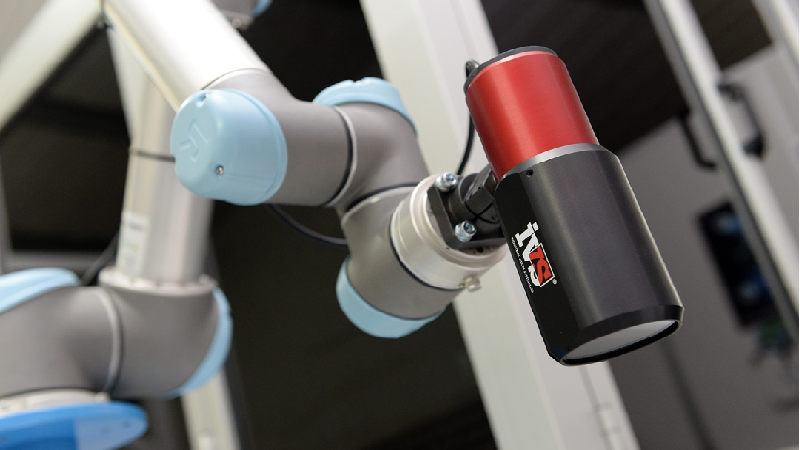
\includegraphics[scale=0.25]{Collaborative-Robot-Inspection.png}
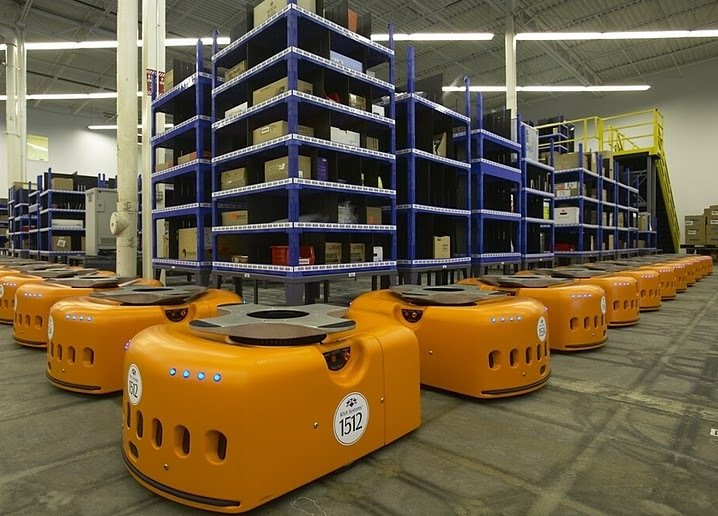
\includegraphics[scale=0.2]{amazonlogistics.jpg}
\caption{Algunas aplicaciones de la robótica: inspección / logística de almacenes}
\label{fig:apps}
\end{center}
\end{figure}

\noindent Otros sectores como el de la logística están siendo transformados a través de robots que se encargan de realizar tareas como el embalaje, transporte o recogida del producto (Figura \ref{fig:apps}). Con esto se pretende, entre otros motivos, satisfacer la exigencia del cliente en términos de entregas rápidas y eficientes. Además de esto existen numerosas aplicaciones que surgen de la unión de Robótica y Visión Artificial, principalmente, que se están comenzando a utilizar en el día a día. Ejemplo de ello es la irrupción completa del coche autónomo en el panorama automovilístico donde se afrontan problemas que van desde la reconstrucción estéreo, la calibración de las cámaras del vehículo hasta la detección de objetos ~\cite{janai2017computer}. Por último, es necesario mencionar una de las aplicaciones más conocidas de la robótica, se trata del robot aspiradora al que ya no es novedad encontrar en muchos hogares (Figura \ref{fig:roomba}).
\begin{figure}[H]
\begin{center}
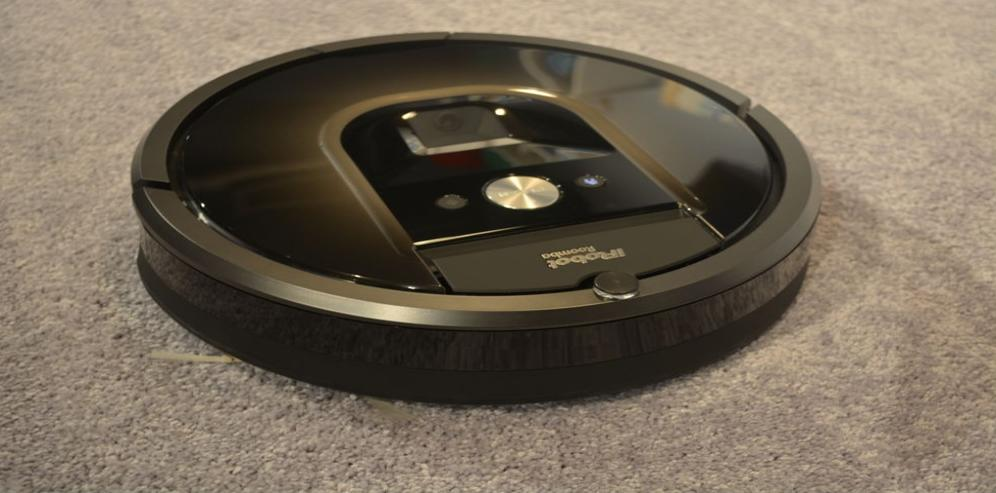
\includegraphics[scale=0.20]{roomba980.jpg}
\caption{Aspiradoras robóticas}
\label{fig:roomba}
\end{center}
\end{figure}
\subsection{Redes Neuronales en Visión Artificial}
Desde el nacimiento de la Inteligencia Artificial (IA) en 1956 la robótica y la visión artificial han seguido un gran ritmo de evolución. Llevando a las máquinas a igualar a los humanos en la resolución de algunas tareas, y en ciertos casos, a superarlos.
La inteligencia artificial se define en ~\cite{mccarthy2006proposal} como "el subcampo de las Ciencias de la Computación dedicado a desarrollar programas que permitan a los ordenadores presentar comportamientos que se puedan caracterizar como inteligentes". El aprendizaje máquina o \textit{Machine Learning} (\textit{ML}) se define en ~\cite{samuel2000some} como "un campo de las Ciencias de la Computación que dá a los ordenadores la capacidad de aprender sin ser explícitamente programados". Por tanto, dada esta definición, el ML se puede considerar un subcampo de la IA.\\
Uno de los subcampos del ML más conocidos y en auge actualmente es el denominado \textit{Deep Learning}~\cite{deng2014deep}. Este tipo de algoritmos se encuentra íntimamente ligado con las Redes Neuronales Artificiales (\textit{ANN}) y en la práctica se suelen usar de forma equivalente aunque no son lo mismo. Uno de los aspectos a destacar en los algoritmos de Deep Learning es que ya no es necesario extraer vectores de características para la entrada a la red. Esto es así porque dichos algoritmos "aprenden" a representar los datos de forma jerárquica. Dentro de estas redes tienen especial interés en la visión artificial y en el problema que afronta este proyecto las redes neuronales convolucionales. Este tipo de redes se caracterizan por utilizar una operación convolución en al menos una de las capas de la red y están diseñadas para el procesado de datos bidimensionales como son las imágenes ~\cite{liu2015implementation}. En los últimos años, su evolución ha sido constante llegando a superar los resultados conseguidos por algoritmos anteriormente en tareas como clasificación o detección de objetos.\\
Para el uso de Deep Learning han surgido numerosos entornos, estos son algunos de los más empleados en la actualidad:
\begin{itemize}
\item \textbf{Tensorflow}: ofrece un API de bajo nivel que permite un control completo sobre los diseños de los modelos y también un API de alto nivel más simplificado pero con una funcionalidad limitada. Además permite la visualización del entrenamiento mediante la herramienta Tensorboard.
\item \textbf{Keras}: proporciona un API de alto nivel para uso de redes de neuronas. Puede correr sobre distintos \textit{backends} como Theano o Tensorflow y dispone modelos de redes pre-entrenadas que permiten crear una red de forma sencilla. Escrita en Python, ofrece un entorno amigable y modular.
\item \textbf{Caffe}: emplea una arquitectura C++/CUDA optimizada para uso en GPU y proporciona interfaces para Python o Matlab, por ejemplo. La definición del modelo se hace mediante Protobuf, formato creado por Google, creando una estructura de datos serializada. También dispone de modelos pre-entrenados e interfaz gráfico.
\item \textbf{Darknet}: este entorno escrito en C y CUDA es rápido y de fácil instalación y proporciona soporte para CPU y GPU. Conocido por su uso en YOLO ~\cite{redmon2016yolo9000}, una de las técnicas del estado del arte en detección de objetos que se comentará posteriormente.
\end{itemize}
En ~\cite{kovalev2016deep} se realiza un estudio comparativo que incluye los tres primeros entornos citados donde se pueden destacar las buenas prestaciones de los mismos respecto a otros.
\subsection{Datasets en Visión Artificial}
Los conjuntos de datos empleados a la hora de implementar un determinado sistema o probarlo son clave pues influyen en el rendimiento que pueda llegar a obtener el mismo. Además permiten hacer una comparativa de la solución encontrada respecto a otras que conforman el Estado del Arte en la tarea que se realiza, pues suelen estar asociados a algún tipo de competición. Por ello es necesario elegir correctamente el dataset o los datasets empleados en un problema de visión artificial. A continuación se comentan algunos de los datasets más relacionados con las tareas que se pretenden realizar en este trabajo:
\begin{itemize}
\item \textbf{COCO (Common Objects in Context)}\footnote {\href{http://cocodataset.org/#home}{COCO Dataset}}: es un dataset de larga escala para detección y segmentación de objetos principalmente. Contiene 80 categorías de objetos y 330000 imágenes de las cuales más de 200000 están etiquetadas. Es un dataset ampliamente utilizado entre la comunidad y en congresos como el ICCV (International Conference on Computer Vision).
\item \textbf{ImageNet}\footnote {\href{http://www.image-net.org/}{ImageNet Dataset}}: este dataset de imágenes consta en la actualidad con 14 millones de imágenes aproximadamente y una media de 500 imágenes por cada categoría o nodo. Organiza el conocido \textit{challenge} ILSVRC de localización y detección de objetos en imágenes y vídeos (hasta el año 2012 en conjunto con PASCAL VOC) y se está convirtiendo en uno de los datasets de referencia en este área.
\item \textbf{Cityscapes}\footnote {\href{https://www.cityscapes-dataset.com/}{Cityscapes Dataset}}: este dataset se centra en la segmentación semántica en escenas urbanas. Contiene 30 clases de objetos, 5000 imágenes etiquetadas con etiqueta \say{fina} (\textit{fine}) y 20000 etiquetadas con etiqueta \say{gruesa} (\textit{coarse}) en 50 ciudades diferentes.
\end{itemize}
Existen numerosos datasets más como INRIA, los datasets del MIT o Caltech, por ejemplo, que contribuyen a la mejora continua en este área.

\subsection{Objetivos}
Como se ha comentado al comienzo de esta sección de introducción el objetivo principal de este trabajo es la implementación de una memoria visual en un robot utilizando para ello redes neuronales. El robot deberá ser capaz de "comprender" el entorno que le rodea detectando clases como humanos, puertas, mesas o ventanas y con esto poder tomar buenas decisiones. Para ello se va a probar el uso de una técnica novedosa dentro del campo de la segmentación semántica conocida como \textit{Mask R-CNN} que ha demostrado resultados prometedores ~\cite{he2017mask}.

%-------------------------------------------------------------------------
\section{Trabajos previos en tracking}
Una vez vistas las bases sobre las que se sustenta el proyecto es necesario ver cuáles han sido y son los trabajos que forman el Estado del Arte en las técnicas que se van a utilizar para resolver el problema que se plantea. Por ello, en esta sección se hablará de métodos de tracking, clasificación, detección y segmentación de objetos.\\
En el campo de la visión artificial existen una gran variedad de áreas de estudio, una de las más importantes es el denominado seguimiento de objetos (\textit{object tracking}). Su objetivo principal es estimar el estado del objeto (\textit{target}) durante el tiempo en una serie de secuencias de imágenes (\textit{frames}). Este estado puede ser definido por diferentes características como la forma, la apariencia, la posición o la velocidad.\\
Se trata de un campo difícil ya que se pueden dar una o más circunstancias que deben ser resueltas por el algoritmo. Entre ellas están el manejo de variaciones en la iluminación y en el punto de vista del objeto que puede llevar a cambios en la apariencia del mismo. Así mismo, las oclusiones que ocurren cuando los objetos se mezclan con otros elementos de la escena o la calidad de la imagen en sí pueden ser un problema a tener en cuenta en este área.\\
Para afrontar estos problemas se han seguido los siguientes paradigmas ~\cite{smeulders2014visual}:
\begin{itemize}
\item \textbf{Tracking using matching}: este grupo de algoritmos hace un \textit{matching} entre la representación del modelo del objeto creado del frame anterior y los posibles candidatos en el siguiente frame. Los métodos más destacados son \textit{Normalized Cross-Correlation} ~\cite{briechle2001template}, \textit{Lucas-Kanade Tracker} ~\cite{baker2004lucas}, \textit{Kalman Appearance Tracker} ~\cite{nguyen2004fast} y \textit{Mean Shift Tracking} ~\cite{comaniciu2000real}.
\item \textbf{Tracking-by-detection}: en estos se construye un modelo para distinguir el objeto del fondo ~\cite{nguyen2006robust}. Una vez se tiene la detección se asocia con las demás detecciones. En la actualidad, la comunidad está girando hacia las redes neuronales para computar las detecciones.
\item \textbf{Tracking, learning and detection}: se trata de una extensión del grupo anterior que incluye un mecanismo para actualizar el modelo que se aprende durante la ejecución. Por ejemplo, se pueden usar los resultados de un \textit{optical flow tracker} para esta actualización ~\cite{kalal2010pn}. Así se consigue que el algoritmo sea invariante ante cambios en el objeto. 
\end{itemize}
Previamente a las técnicas modernas que se van a comentar existen formas más clásicas de hacer seguimiento de objetos y que pueden ser útiles en problemas que exijan tiempo real a la hora de realizar el tracking, por ejemplo. Una de las más conocidas es el \textit{feature tracking}. Esta técnica emplea puntos característicos que se puedan encontrar en las imágenes y permitan estimar el movimiento. Estos puntos deben de cumplir unos requerimientos para poder ser característicos de la imagen como son la repetibilidad (la característica se podrá encontrar en las imágenes aunque estas hayan sufrido alguna transformación), la compatibilidad (cada característica debe de ser descriptiva y fácil de encontrar) o la eficiencia (la representación de la información característica de la imagen se debe realizar con el menor número de características posible). Unos de los puntos característicos más utilizados son las esquinas que se caracterizan por gradientes con valor más alto en ellas en dos o más direcciones. Entre estas técnicas se destacan los puntos de Harris~\cite{harris1988combined} y Shi-Tomasi~\cite{shi1994good}.\\
Existen sistemas de tracking que aprovechan la rapidez del feature tracking y el acierto de las redes neuronales para crear un tracking híbrido. En él se realizan las detecciones cada N frames utilizando algún tipo de red neuronal y el seguimiento intermedio se realiza mediante feature tracking.\\
Con la llegada de las redes neuronales esta forma de agrupar los diferentes métodos de tracking cambia para adaptarse a ellas ~\cite{held2016learning}:
\begin{itemize}
\item \textbf{Tracking-by-detection}: están diseñados para seguir una determinada clase de objetos (\textit{model-based}) y obtener un clasificador específico. En fase de test las detecciones obtenidas con redes neuronales son vinculadas usando información temporal. Se encuentran limitados a una sola clase de objetos.
\item \textbf{Tracking, learning and detection}: se caracterizan por ser entrenados completamente \textit{online}. Un ejemplo típico de tracker de este grupo muestrea zonas cercanas al objeto y las considera "\textit{foreground}", lo mismo ocurre con las zonas lejanas que serían asignadas al "\textit{background}". Con esto permite construir un clasificador que los diferencie y estimar la nueva localización del objeto en el siguiente frame ~\cite{babenko2009visual}. Se ha probado a introducir redes neuronales en entornos con entrenamiento online pero debido a la lentitud de las redes a la hora de entrenar los resultados son lentos en fase de test.
\item \textbf{Siamese-based tracking}: usando técnicas de \textit{patch-matching} ~\cite{tao2016siamese} en este tipo de redes se reciben múltiples patch candidatos del nuevo frame y se escoge como mejor candidato aquel con mayor \textit{matching score} respecto al frame anterior, es decir, el más similar según la función de matching.
\item \textbf{Tracking as regression}: en este grupo, en cambio, la red recibe solamente dos imágenes y regresa directamente la localización del objeto ~\cite{held2016learning}.
\item \textbf{Tracking con RNN}: a partir de la detección obtenida este tipo de algoritmos emplean \textit{Recurrent Neural Networks} para modelar la secuencia del movimiento de los objetos mejorando así la respuesta a oclusiones prolongadas en el tiempo, por ejemplo ~\cite{sadeghian2017tracking}. Son el estado del arte en tracking en la actualidad.
\end{itemize}
\section{Trabajos previos en clasificación y detección usando redes neuronales}
Mucho del progreso realizado durante los últimos años en la clasificación en visión artificial se puede asociar directamente a un conjunto de arquitecturas de redes neuronales. Gran parte de las mismas vienen implementadas y entrenadas en Keras\footnote {\href{https://keras.io/applications/}{Keras Applications}}: VGG16, VGG19, ResNet50, Inception v3, Xception o MobileNet, son algunas de ellas.\\ Pero el primer gran paso adelante vino en 2012 cuando AlexNet ~\cite{krizhevsky2012imagenet} bate todas las propuestas del estado del arte en ese momento en el concurso (\textit{challenge}) de ImageNet, ILSVRC, un challenge de clasificación en imágenes de referencia en visión artificial en la actualidad. AlexNet obtuvo una tasa de error en test del 15,3\% en comparación con el ganador el año anterior que fue del 26,2\%. Esta red, junto con las redes VGG ~\cite{simonyan2014very}, sigue el arquetipo de diseño básico de las redes convolucionales: una serie de capas de convoluciones, seguido de max-pooling y capas de activación antes de las capas finales de clasificación \textit{fully-connected}. MobileNet es una versión simplificada de Xception ~\cite{chollet2016xception} para aplicaciones móviles que en la actualidad está debajo de las aplicaciones de visión usadas en los dispositivos móviles de Google.\\
Las arquitecturas ResNet e Inception, principalmente, se han convertido en bloques que sirven de base para numerosos trabajos posteriores en visión artificial y se comentan a continuación:
\begin{itemize}
\item \textbf{Res-Net} ~\cite{he2016deep}: esta red trata de resolver el problema que parece aparecer al añadir capas a una red y es que esta se comporta peor generalmente. Por ello, los autores en lugar de tratar de aprender el \textit{mapping} oculto de x a H(x), aprenden la diferencia entre los dos, esto es, el residuo (\textit{residual net}). Y para calcular H(x) simplemente añaden el residuo a la entrada y vuelve a entrar en la siguiente capa.\\ Esto supone un gran cambio en su momento ya que soluciona el problema de los \textit{vanishing gradients} que sufrían las redes neuronales hasta la fecha. Además permite crear redes mucho más profundas, es decir, con más capas, que tengan buenos resultados. Con ello ResNet gana el ILSVRC de 2015 con una tasa de error del 3,57\%.
\item \textbf{Inception} ~\cite{szegedy2015going}: esta familia de redes busca redes más \say{anchas}, esto es, con más operaciones intermedias entre capas. Los autores tratan de aumentar las redes neuronales sin un incremento del coste computacional. Introduciendo diferentes operaciones de convolución en paralelo incrementan la densidad de información extraída pero también los costes computacionales. Para resolver el problema usan convoluciones de 1x1 para reducir la dimensionalidad a la vez que realizan diferentes transformaciones en paralelo. Obteniendo como resultado redes que son simultáneamente profundas y anchas.\\
La primera versión de Inception, conocida como GoogLeNet, fue la ganadora del ILSVRC de 2014. Posteriormente se ha mejorado en Inception v2 y v3 hasta la última versión de Inception, v4. Inception v4 crea un híbrido con ResNet, Inception-ResNet ~\cite{szegedy2017inception}.
\end{itemize}
Con la llegada de los vehículos autónomos, la videovigilancia inteligente, la detección facial y numerosas aplicaciones que están surgiendo, se demanda cada vez unos sistemas de detección más rápidos y precisos. Esto no sólo incluye reconocer y clasificar cada objeto en la imagen sino también localizarlo con su correspondiente \textit{bounding box}. Esto hace de la detección de objetos una tarea significativamente más complicada que la tradicional clasificación de imágenes. A pesar de ello, los algoritmos de detección de objetos más exitosos en la actualidad son extensiones de modelos de clasificación de imágenes.\\
A continuación, se van a introducir los principales modelos de detección de objetos ~\cite{fu2017dssd}.
\begin{itemize}
\item \textbf{Faster R-CNN} ~\cite{ren2015faster}: es uno de los modelos actuales de referencia y uno de los últimos detectores conocidos como \textit{region-based} de Girshick \etal{} Estos modelos funcionan básicamente de la siguiente forma: usan algún mecanismo para extraer regiones de una imagen que probablemente sean un objeto y luego clasifican esas regiones propuestas con una CNN.\\ El padre de este modelo es el R-CNN y fue el verdadero impulsor de este tipo de técnicas ~\cite{girshick2014rich}. En las regiones propuestas obtenidas mediante un algoritmo denominado \textit{Selective Search} se extraen las características mediante una CNN por región y luego se clasifican esas regiones basándose en las características. Pero su funcionamiento era lento.\\
Se mejora llega con Fast R-CNN ~\cite{girshick2015fast} con dos motivos principales. El primero es que se aplica la CNN sobre toda la imagen en lugar de por cada región y luego se obtienen las regiones a partir del último mapa de características de la red. El segundo se debe a la introducción de una capa de Softmax que simplifica la clasificación. Su funcionamiento era más rápido y fácil de entrenar que R-CNN pero aún existía un cuello de botella en la generación de regiones.\\
Para resolverlo se introduce la RPN (\textit{Region Proposal Network}) que sumado al Fast R-CNN crea Faster R-CNN. La RPN devuelve regiones propuestas basándose en un \textit{score} que hace referencia a la probabilidad de que la bounding box sea un objeto (Figura \ref{fig:fasterrcnn}). Y estas regiones son pasadas directamente a la Fast R-CNN.\\
\begin{figure}[h!]
\begin{center}
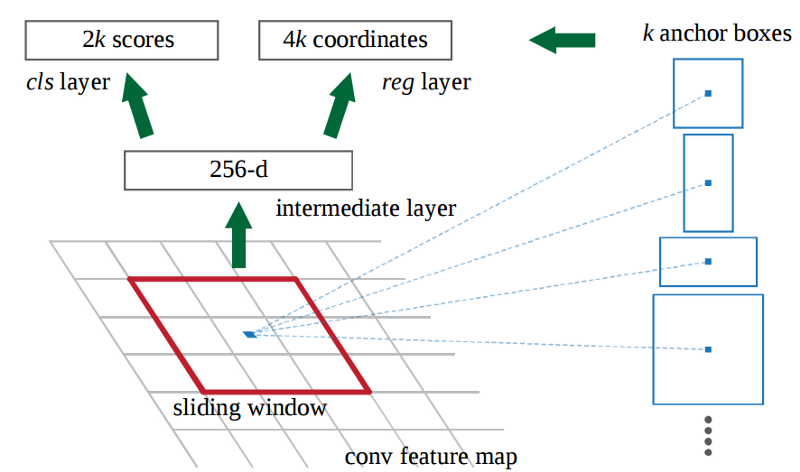
\includegraphics[scale=0.25]{faster_rcnn.png}
\caption{Region Proposal Network (RPN)}
\label{fig:fasterrcnn}
\end{center}
\end{figure}
\item \textbf{Overfeat} ~\cite{sermanet2013overfeat}: ganador del ILSVRC del 2013 en localización y detección de objetos, este trabajo mostró que entrenar una red convolucional para simultáneamente clasificar, localizar y detectar objetos en imágenes puede potenciar el acierto tanto en clasificación como en detección y localización. Posteriormente, ha sido reemplazado por SSD y YOLO para tareas que requieran una mejor detección en tiempo real.
\item \textbf{SSD} ~\cite{liu2016ssd}: existen modelos más rápidos que Faster R-CNN como R-FCN, que trata de mejorar la velocidad del sistema maximizando el cómputo compartido ~\cite{dai2016r}, o SSD. Esta última proporciona grandes ganancias en velocidad respecto a Faster R-CNN realizando las fases de generación de regiones de interés y posterior clasificación de forma conjunta (\textit{Single Shot MultiBox Detector}). Como resultado obtiene una gran cantidad de bounding box de las cuales la mayoría no son útiles. Aplicando en ellas las técnicas \textit{non-maximum suppression} y \textit{hard-negative mining} se consiguen las detecciones finales.
\item \textbf{YOLO} ~\cite{redmon2016yolo9000}: este sistema usa un enfoque diferente a los anteriores ya que aplica una sola red neuronal a la imagen completa. Esta red divide la imagen en regiones y predice los bounding box y probabilidades de cada región. Posteriormente estas son ponderadas con las probabilidades para obtener las detecciones definitivas. Esto lo hace, según indican los autores, cien veces más rápido que Fast R-CNN, por ejemplo, manteniendo un acierto similar. En la última versión, YOLOv2, se introducen algunas mejoras como FCN.
\end{itemize}
En la siguiente tabla obtenida de~\cite{redmon2016yolo9000} se puede observar como YOLO se encuentra casi a la par en acierto con métodos como SSD o Faster R-CNN, mejores en acierto. En cambio, tiene un mejor equilibrio rapidez-acierto ya que consigue trabajar en algunos casos a 91 FPS (\textit{frames per second}) cuando Faster R-CNN apenas llega a 10 FPS (ver Tabla 3 en ~\cite{redmon2016yolo9000}).
\begin{table}[h!]
\begin{center}
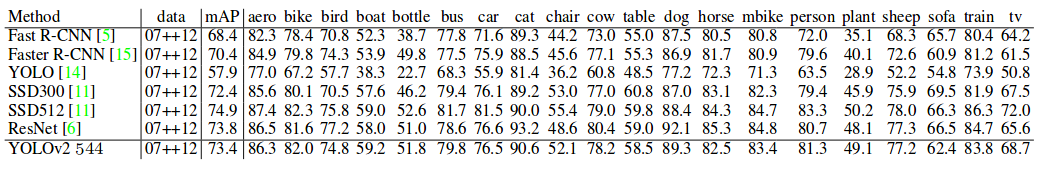
\includegraphics[scale=0.35]{yolo_results_pascal12.png}
\caption{Comparativa de acierto en detección en test de PASCAL VOC 2012}
\end{center}
\end{table}
\section{Trabajos previos en segmentación usando redes neuronales}
La comunidad en visión artificial ha mejorado los resultados obtenidos en detección de objetos y segmentación semántica en un corto período de tiempo gracias, en gran parte, a poderosos sistemas de base como Faster R-CNN. En este proyecto se tratará de realizar segmentación de instancias, lo cual requiere de la correcta detección de todos los objetos en la imagen junto con la segmentación precisa de cada instancia. Así, cada píxel pertenece a alguna de las diferentes categorías sin diferenciar que se encuentre o no en un determinado objeto.\\
Llevados por la efectividad de la familia de R-CNN muchos de los métodos propuestos para segmentación de instancias están basados en propuestas de segmento, donde la segmentación precede al reconocimiento del tipo de objeto ~\cite{pinheiro2015learning}. Esto ha demostrado ser más lento e impreciso que si se realizase de forma paralela y separada la predicción de las máscaras del objeto y las etiquetas de las clases. Li \etal{} proponen un sistema conocido como FCIS (\textit{Fully Convolutional Instance Segmentation}) ~\cite{li2016fully} que trata de predecir la salida de un conjunto de canales sensibles a la posición de forma completamente convolucional. Estos canales realizan las tareas de obtención de las clases, bounding box y máscaras de forma simultánea lo que los hace más rápidos, pero muestran errores en instancias que se solapan creando bordes espurios de forma sistemática (Figura \ref{fig:fcis_mask}).\\
Recientemente surge Mask R-CNN ~\cite{he2017mask} para resolver muchos de estos problemas y situarse como técnica estado del arte en segmentación de instancias como se puede ver en la Figura \ref{fig:fcis_mask}. Por ello esta sección se va a centrar en esta técnica y sus resultados.\\
\begin{figure}[H]
\begin{center}
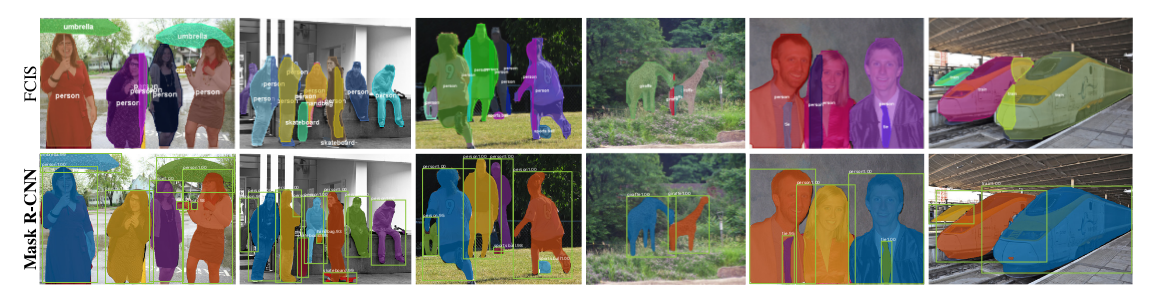
\includegraphics[scale=0.30]{fcis_vs_maskrcnn.png}
\caption{Resultados obtenidos por FCIS y Mask R-CNN en imágenes de test de COCO Dataset}
\label{fig:fcis_mask}
\end{center}
\end{figure}
Conceptualmente, Mask R-CNN añade una tercera etapa a Faster R-CNN en la que obtiene la máscara del objeto. La primera etapa de RPN coincide con la de Faster R-CNN mientras que en la segunda calcula, en paralelo con la predicción de la clase y la bounding box, una máscara binaria para cada región de interés (RoI). La generación de máscaras para cada clase se hace sin que las clases compitan entre ellas lo que permite separar la máscara y la predicción de la clase del objeto. Según los autores, esto demuestra ser clave para unos buenos resultados en la segmentación final.\\ 
Otro de los factores clave en el buen funcionamiento de este método es el alineamiento correcto entre las RoI y las características extraídas. Esto se suele hacer mediante \textit{RoIPool} en Fast R-CNN pero introduce desalineamientos si lo que se desea es segmentar en lugar de clasificar, por lo que en Mask R-CNN se crea \textit{RoIAlign} para corregir este problema. Para demostrar la generalidad del método propuesto los autores introducen la rama de predicción de la máscara sobre varias arquitecturas de redes neuronales existentes como Faster R-CNN con ResNet como extractor de características, por ejemplo, y logran superar a los ganadores del COCO Challenge de segmentación de 2015 y 2016, MNC~\cite{dai2016instance} y FCIS~\cite{li2016fully}. En estos experimentos se utilizan las métricas \textit{standard} de COCO.
\begin{table}[h!]
\begin{center}
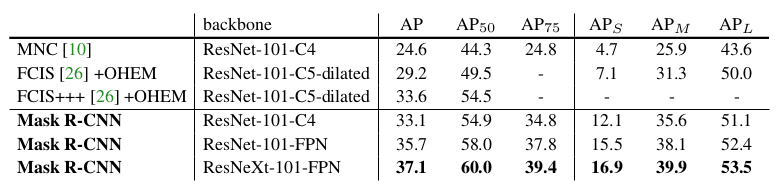
\includegraphics[scale=0.40]{mask_vs_mnc_fcis.png}
\caption{Resultados obtenidos por Mask R-CNN vs el estado del arte en segmentación hasta el momento en imágenes de test de COCO Dataset}
\end{center}
\end{table}
Como se aprecia, todas las implementaciones del modelo Mask R-CNN superan los modelos base previos del estado del arte en segmentación de instancias.\\
Los autores también han realizado experimentos del rendimiento de esta técnica en el dataset Cityscapes (comentado en la sección 1.3). Para las categorías \textit{persona} y \textit{coche} este dataset presenta un gran número de instancias de diferentes clases solapadas, esto hace aún más complicada la correcta segmentación de instancias. Sin embargo, Mask R-CNN mejora los mejores métodos actuales en esta tarea y se convierte en método estado del arte.
%------------------------------------------------------------------------
\bibliography{egbib}{}

\end{document}
